\documentclass[a4paper, 11pt]{report}
\usepackage[a4paper, margin=2.5cm]{geometry}

% Police
\usepackage{libertine}

% Interlignes et paragraphes
\usepackage{setspace} % pour l'interligne
\usepackage{parskip}  % pour gérer l'espacement entre les paragraphes

% Interligne multiple de 1.15
\setstretch{1.15}

% Espace après paragraphe : 6pt
\setlength{\parskip}{6pt}
\setlength{\parindent}{15pt} % Retrait en début de paragraphe

\usepackage{lmodern}
\usepackage[french]{babel}
\usepackage[utf8]{inputenc}
\usepackage[T1]{fontenc}

\usepackage{graphicx} % Pour les images
\graphicspath{Figures}
\usepackage{caption}
\usepackage{siunitx} % for S column in tabular
\usepackage{subcaption}
\usepackage{amsmath, amsfonts, amssymb} %Pour les maths

\usepackage{textcase}

\usepackage{afterpage}

% La numérotation

\makeatletter\@addtoreset{section}{chapter}\makeatother
\renewcommand{\thepart}{\Roman{part}}
\renewcommand{\thechapter}{\arabic{chapter}}
\renewcommand{\thesection}{\Roman{section}}

\usepackage{chngcntr}
\counterwithin{figure}{section}

% Sommaire + hyperliens

\usepackage[hyphens]{url}
\usepackage[pdfauthor = {{Julien Sagnes}}, pdftitle = {{Rapport de Projet}}, pdfstartview = Fit, pdfpagelayout = SinglePage, pdfnewwindow = true, bookmarksnumbered = true, breaklinks, colorlinks, linkcolor = black, urlcolor = black, citecolor = black, linktoc = all]{hyperref}
\usepackage[
    left = \flqq{},% 
    right = \frqq{},% 
    leftsub = \flq{},% 
    rightsub = \frq{} %
]{dirtytalk} % permet de citer mieux

% Codes

\usepackage{booktabs}
\usepackage{listings}
\usepackage{xcolor}
\usepackage[section]{placeins}
\usepackage{enumitem}
\usepackage{accsupp}

\newcommand{\noncopynumber}[1]{%
    \BeginAccSupp{method=escape,ActualText={}}%
    #1%
    \EndAccSupp{}%
}

\definecolor{codegreen}{rgb}{0,0.6,0}
\definecolor{codegray}{rgb}{0.5,0.5,0.5}
\definecolor{codepurple}{rgb}{0.58,0,0.82}
\definecolor{backcolour}{rgb}{0.95,0.95,0.92}

\lstdefinestyle{mystyle}{
    backgroundcolor=\color{backcolour},   
    commentstyle=\color{codegreen},
    keywordstyle=\color{magenta},
    numberstyle=\tiny\color{codegray},
    stringstyle=\color{codepurple},
    basicstyle=\ttfamily\footnotesize,
    breakatwhitespace=false,         
    breaklines=true,                 
    captionpos=b,                    
    keepspaces=true,                 
    numbers = left,
    numberstyle=\tiny\noncopynumber,
    numbersep=5pt,                  
    showspaces=false,                
    showstringspaces=false,
    showtabs=false,                  
    tabsize=2,
    literate=
  {á}{{\'a}}1 {é}{{\'e}}1 {í}{{\'i}}1 {ó}{{\'o}}1 {ú}{{\'u}}1
  {Á}{{\'A}}1 {É}{{\'E}}1 {Í}{{\'I}}1 {Ó}{{\'O}}1 {Ú}{{\'U}}1
  {à}{{\`a}}1 {è}{{\`e}}1 {ì}{{\`i}}1 {ò}{{\`o}}1 {ù}{{\`u}}1
  {À}{{\`A}}1 {È}{{\'E}}1 {Ì}{{\`I}}1 {Ò}{{\`O}}1 {Ù}{{\`U}}1
  {ä}{{\"a}}1 {ë}{{\"e}}1 {ï}{{\"i}}1 {ö}{{\"o}}1 {ü}{{\"u}}1
  {Ä}{{\"A}}1 {Ë}{{\"E}}1 {Ï}{{\"I}}1 {Ö}{{\"O}}1 {Ü}{{\"U}}1
  {â}{{\^a}}1 {ê}{{\^e}}1 {î}{{\^i}}1 {ô}{{\^o}}1 {û}{{\^u}}1
  {Â}{{\^A}}1 {Ê}{{\^E}}1 {Î}{{\^I}}1 {Ô}{{\^O}}1 {Û}{{\^U}}1
  {œ}{{\oe}}1 {Œ}{{\OE}}1 {æ}{{\ae}}1 {Æ}{{\AE}}1 {ß}{{\ss}}1
  {ű}{{\H{u}}}1 {Ű}{{\H{U}}}1 {ő}{{\H{o}}}1 {Ő}{{\H{O}}}1
  {ç}{{\c c}}1 {Ç}{{\c C}}1 {ø}{{\o}}1 {å}{{\r a}}1 {Å}{{\r A}}1
  {€}{{\EUR}}1 {£}{{\pounds}}1
}
\lstset{style=mystyle}

\begin{document}

\definecolor{darkWhite}{rgb}{0.94,0.94,0.94}

% Page de garde

\begin{titlepage}
    \newcommand{\HRule}{\rule{\linewidth}{0.5mm}}
    \begin{center}
        \begin{minipage}{1\linewidth}
            \begin{flushleft}
                \hspace{4.5cm}
                
\includegraphics[width=0.25\textwidth]{Figures/SORBONNE_FAC_SCIENCES_DEF_CMJN.pdf}
            \end{flushleft}
        \end{minipage}

        \vspace{1.5cm}
        
        \textsc{\Large{}Master SAR 1\up{\MakeTextLowercase{ère}} année} \\[0.5cm]
        \textsc{\large{}2024 - 2025} \\[0.5cm]

        \HRule \\[0.6cm]
        {\huge\bfseries{}Rapport de projet :} \\
        \LARGE{Conception et dimensionnement d'une pince robotique à trois doigts flexibles} \\[0.25cm]
        \HRule \\[1.5cm]


        \Large\textit{Auteurs :}\\
        \begin{center}
            Julien \textsc{Sagnes}\\
            Minh \textsc{Nhut Nguyen}
        \end{center}

        \hfill

        \Large\textit{Responsable :}\\
        \begin{center}
            Faiz \textsc{Ben Amar}
        \end{center}
        \vspace{1cm}
        {\large\today} \\[2cm]
    \end{center}

    \vfill
\end{titlepage}


\selectlanguage{french}
% Résumé sur une page séparée avant la table des matières
\clearpage
\section*{Résumé}
\addcontentsline{toc}{section}{Résumé}
Ce document présente la conception et le dimensionnement d'une pince robotique à trois doigts flexibles. Blablabla...

\clearpage
\tableofcontents
\clearpage

\section{Introduction}

    Dans l'indurainure, la robotique collaborative, ou cobotique, est omniprésente. Elle vise à soulager l’être humain en prenant en charge les tâches pénibles, notamment à l’aide de préhenseurs conçus spécifiquement pour manipuler des charges de tailles et de poids variables, souvent associées à des tâches répétitives. \cite{noauthor_cobotique_nodate}

    Ce projet consiste à concevoir et dimensionner une pince robotique à trois doigts flexibles, conçue pour s'ouvrir et se refermer en s'adaptant à l'objet saisi. L'objectif est de réussir à attraper des fruits et légumes relativement légers, comme un poivron. Nous utiliserons \textit{SolidWorks} pour modéliser le robot, et étudierons son élasticité par éléments finis via \textit{SolidWorks Simulation}.

    Elle sera ensuite fixé au bras robotique...

    \subsection{Motivations et principes fondamentaux}

        \begin{figure}
            \centering
            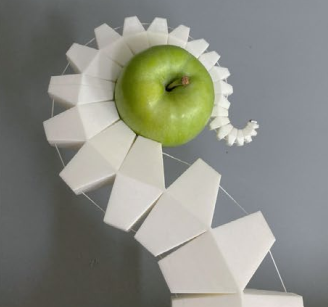
\includegraphics[width=0.5\textwidth]{Figures/pieuvre.png}
            \caption{Inspiration du SpiRob pour les 3 doigts de notre pince \cite{wang_spirobs_2025}}
            \label{fig:pieuvre}
        \end{figure}
    
        Dans notre cas, et comme souvent en robotique, les objets à manipuler ont une forme ou une position mal connue, et contrairement à une main humaine, les pinces robotiques manquent de retour tactile fiable. Pour cette raison, nous n'allons pas utiliser de retour haptique, mais plutôt de préhenseurs souples. Nous nous inspirons de la flexibilité des tentacules de pieuvre (voir figure \ref{fig:pieuvre}), ce qui permettra à la pince de s'adapter naturellement à la forme de divers fruits et légumes, sans nécessiter de capteurs ni de système de contrôle complexe, grâce à la compliance mécanique.
        
        La compliance désigne la capacité d’un robot à adapter la rigidité de ses mouvements en fonction des forces extérieures. Autrement dit, il ajuste naturellement sa posture pour bien épouser l’objet qu’il manipule. Dans ce projet, nous nous concentrons sur la compliance passive, où la structure mécanique du robot est suffisamment flexible pour se déformer sous l'effet d'une contrainte externe. Cette approche permet une préhension polyvalente et adaptable. \cite{noauthor_gestion_2016}

        Malgré ses avantages, cette flexibilité favorise le flambage sous de grandes forces d'actionnement et limite donc la charge maximale. Il faut donc établir un compromis sur la souplesse, afin d'assurer la flexibilité et la capacité à soutenir des charges raisonnables. \cite{wang_spirobs_2025}
    
    \subsection{Comportement et structure de la pince}
    
        La pince pourra adopter deux configurations distinctes : ouverte ou fermée. Elle sera haute de 10 cm en position ouverte et composée de 3 doigts identiques soumis à un encastrement rigide sur une base. Les doigts seront positionnés symétriquement autour du centre de la base, chacun séparé par un angle de 120°. Des câbles passeront de chaque côté des doigts et permettront de les contrôler. L'actionnement à câbles peut être localisé sur les effecteurs ou déporté sur la base, il sera question d'effectuer une étude comparative des différentes solutions possibles.
        
        La flexion de chaque doigt sera assurée par une force appliquée sur le câble situé du côté fléchisseur par l'utilisation d'un moteur, tandis que le retour à la position initiale se fera naturellement, cette dernière devant être la position d'équilibre lorsque le moteur n'exerce plus de couple. Il est donc crucial de dimensionner correctement les doigts et les câbles afin qu'ils conservent un comportement élastique et réversible, sans déformation permanente. C'est pourquoi nous utiliserons un matériau souple qui puisse se plier sans se casser, le TPU.
        
        ((Par la suite, nous étudierons les flexions, les contraintes maximales et le retour élastique afin de s'assurer de ne pas rentrer dans le modèle élastique.))
                
        Enfin, il sera essentiel de garantir autant que possible la répétabilité, un aspect souvent problématique dans le domaine de la robotique flexible, car la souplesse peut introduire des incertitudes sur la position exacte des doigts.

    \subsection{Choix de l'actionneur}

        Il sera question de choisir entre un moteur rotatif qui actionnerait un tambour ou un moteur linéaire. En tout cas, un seul moteur doit synchroniser l'ouverture/fermeture des 3 doigts. On se donne pour cahier des charges de pouvoir soulever des objets de l'ordre de 5 kilogrammes. Il a été choisi de faire par un moteur rotatif, car nous avions en laboratoire.

\clearpage

\section{État de l'art des préhenseurs souples et leurs actionneurs}

    \subsection{Préhenseurs souples}
    
        \subsubsection{Étude d'une pince en PVC}
            
            \begin{figure}[htbp]
                    \centering
                    \begin{subfigure}[t]{0.8\textwidth}
                        \centering
                        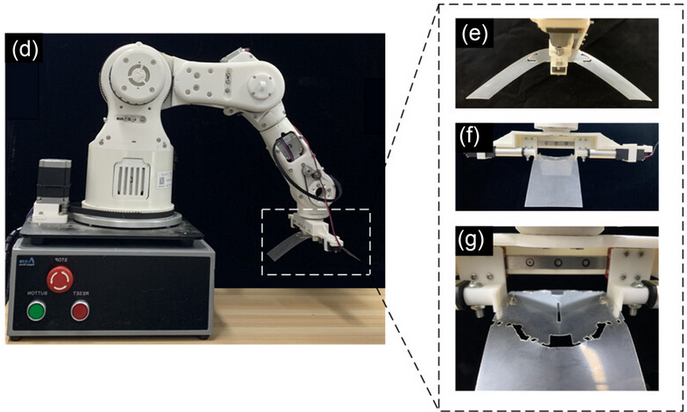
\includegraphics[width=\textwidth]{Figures/robot.png}
                        \caption{Robot Anno V6-PLUS qui porte la pince \cite{liu_origami_2023}}
                    \end{subfigure}
                    \hfill
                    \begin{subfigure}[t]{0.8\textwidth}
                        \centering
                        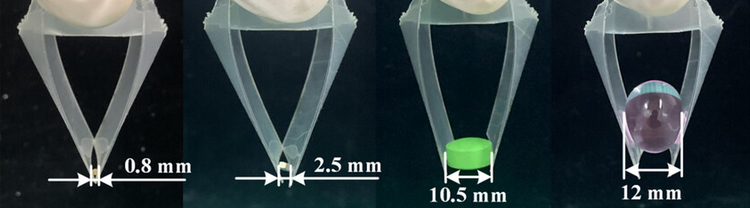
\includegraphics[width=\textwidth]{Figures/adaptability.png}
                        \caption{Exemples d'utilisation de la pince souple \cite{liu_origami_2023}}
                    \end{subfigure}
                    \caption{Illustration de l'étude sur la pince souple}
                    \label{fig:origami}
                \end{figure}
        
            Une étude a été menée afin de concevoir des préhenseurs souples en origami, permettant une adaptabilité de préhension pour de nombreux objets. La pince, qui n'est qu'une simple feuille de PVC (voir figure \ref{fig:origami}.a.(e)), est commandée grâce à un moteur linéaire. Le moteur linéaire est fixé au bras robotique via un support (bracket). Ce moteur est relié à un poussoir qui coulisse sur une glissière. Lorsqu’on alimente le moteur linéaire, il pousse ou tire le poussoir de manière rectiligne. Le mouvement du poussoir est ainsi transmis à la pince flexible, qui s’ouvre ou se ferme selon la direction du mouvement. Afin de garantir la stabilité, un cadre de limitation empêche le poussoir de dépasser certaines positions, et le système de guidage symétrique (les deux extrémités du poussoir étant à la même hauteur) empêche la pince de se déformer de manière asymétrique, ce qui garantit une prise stable (voir figure \ref{fig:origami}.a.(g)). \cite{liu_origami_2023}.
    
            Cette étude nous permet de voir l'adaptabilité remarquable que permettent les préhenseurs souples. En effet, comme nous pouvons le remarquer sur la figure \ref{fig:origami}.b, la pince souple s'adapte parfaitement à chaque taille d'objet pour le même effort à son extrémité.

        \subsubsection{Étude d'une pince flexible multi-stable à l'aide du kirigami}
    
            \begin{figure}
                \centering
                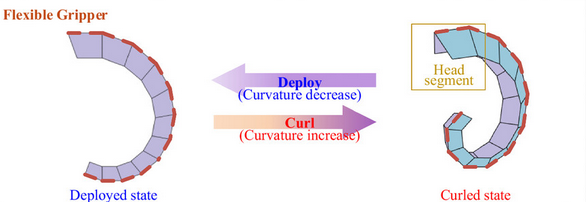
\includegraphics[width=0.7\textwidth]{Figures/multi-stable.png}
                \caption{Pince à plusieurs positions stables \cite{qi_kirigami_2024}}
                \label{fig:multi_stable}
            \end{figure}
    
            Cette étude \cite{qi_kirigami_2024} explore la conception d'une pince souple en s'appuyant sur les principes du kirigami, une technique dérivée de l'origami. Cette approche permet de générer des structures à multi-stabilité passive, c’est-à-dire capables de maintenir plusieurs configurations d’équilibre, notamment une configuration pince fermée et une autre pince ouverte (voir figure \ref{fig:multi_stable}). Ce changement de configuration s'opère grâce à une structure "trigger" (déclencheuse) capable de convertir une force longitudinale appliquée en un mouvement de déformation latérale des bras de la pince.
    
            Néanmoins, l’approche présente aussi des limites, notamment en termes de force de préhension. La pince kirigami décrite utilise des actionneurs diélectriques ou des forces manuelles pour effectuer la transition de forme, ce qui restreint sa capacité à soulever des charges importantes. Cela la rend peu adaptée aux applications où une capacité de charge élevée est requise — comme c’est le cas dans notre projet où l’objectif est de manipuler des objets jusqu’à 5 kg. Enfin, bien que le système ne repose pas sur une action par câble comme notre pince inspirée du SpiRob, cette étude permet de souligner que les principes de déformation géométrique contrôlée et de multi-stabilité passive constituent une piste intéressante pour notre pince.
    
        \subsubsection{Étude de la spirale logarithmique avec le SpiRob}
        
            \begin{figure}
                \centering
                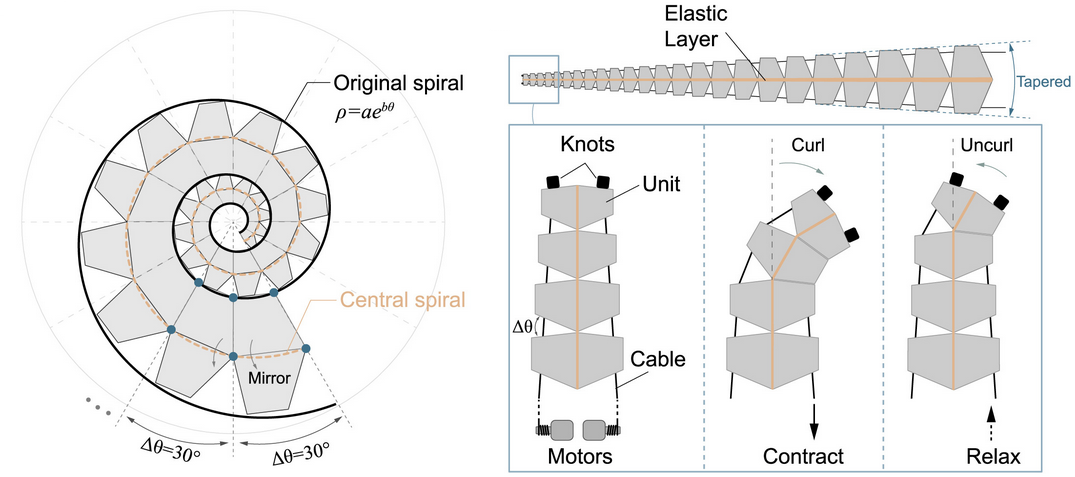
\includegraphics[width=1.0\textwidth]{Figures/spiral_logarithm.png}
                \caption{Spiral logarithmique du préhenseur \cite{wang_spirobs_2025}}
                \label{fig:spiral_logarithm}
            \end{figure}
    
            On remarque alors le lien avec la spirale logarithmique, dont on reproduit la forme à l'aide d'un matériau souple. On commande ensuite le robot avec une force exercée sur les câbles de chaque côté du bras à l'aide d'un moteur. Cette stratégie capitalise spécifiquement sur la déformation passive au contact pour s'adapter à des objets de formes et de tailles variables (voir figure \ref{fig:pieuvre}).

            Pour notre projet, nous choisissons cette approche.

        \subsection{Actionneurs}

            \subsubsection{Étude des systèmes de transmissions et d'actionnements par câble pour des exosuits. }

\clearpage
        
\section{Conception de la pince}
        
    \subsection{Considérations mathématiques}

        \subsubsection{Spirale centrale}
            
            Sur la figure \ref{fig:spiral_logarithm}, la spirale centrale qui définit notre robot vérifie la relation :
            \begin{equation}
            r_c(\theta) = \frac{r(\theta) + r(\theta + 2\pi)}{2}, \quad \forall \theta
            \label{eq:spirale_centrale}
            \end{equation}
            
            Cela signifie qu’on prend le rayon au point $\theta$ ($r(\theta)$), celui au point $\theta + 2\pi$ ($r(\theta + 2\pi)$), et on calcule leur moyenne. Cela donne un point « central » pour chaque angle $\theta$, et en les reliant, on forme la spirale centrale. \cite{wang_spirobs_2025}

        \subsubsection{Choix et détermination des coefficients}

            \begin{figure}
                \centering
                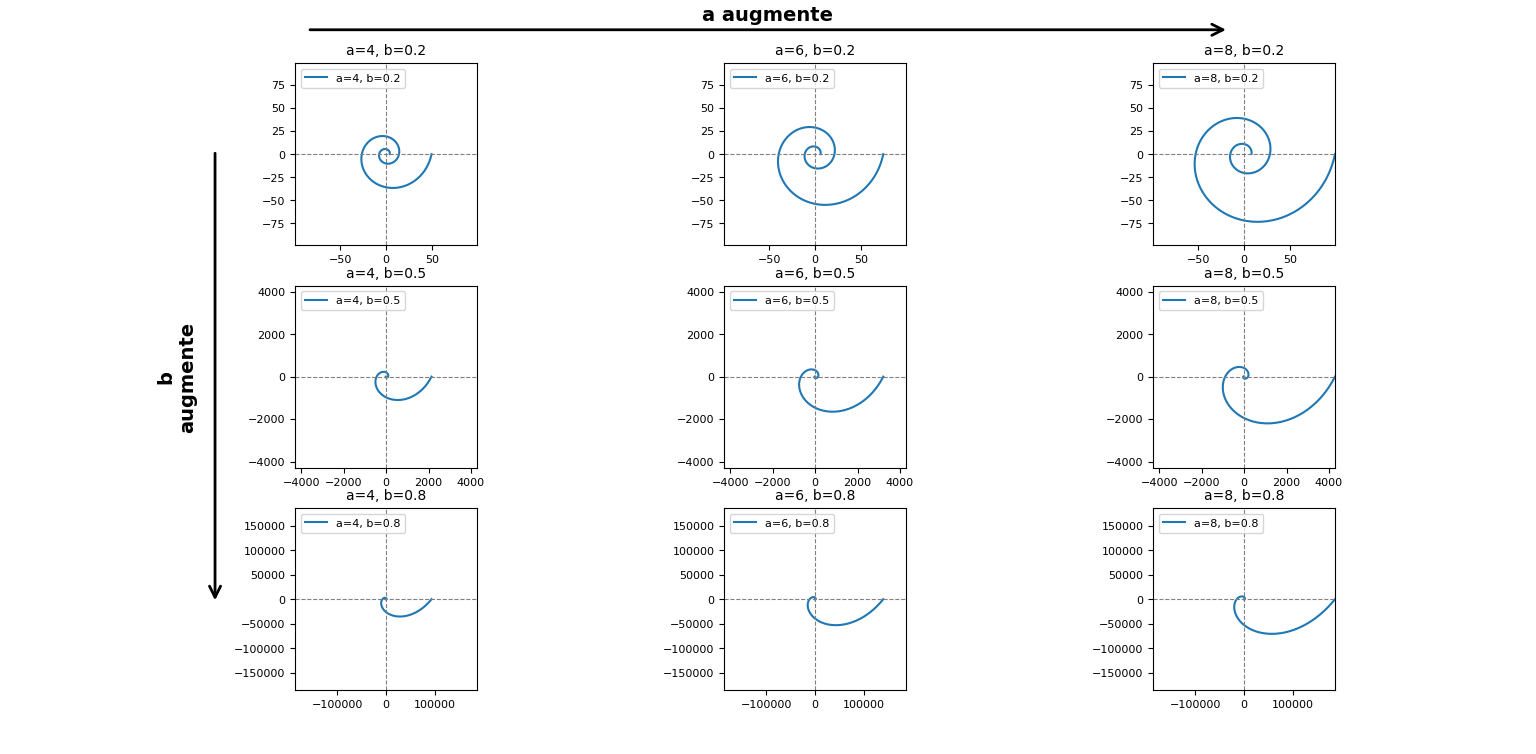
\includegraphics[width=1\textwidth]{Figures/spirale.png}
                \caption{Influence des coefficients $a$ et $b$ sur le tracé de la spirale logarithmique}
                \label{fig:spirale}
            \end{figure}
        
            Dans \cite{wang_spirobs_2025}, les auteurs expliquent comment dessiner le SpiRob. Nous nous inspirons de sa forme pour concevoir nos doigts.
        
            La spirale logarithmique est d'équation en coordonnées polaires ($r, \theta$) :
            \begin{equation}
            r = ae^{b\theta}, \quad \text{avec} \quad a > 0
            \label{eq:spirale_log}
            \end{equation}
            
            Sachant que $a$ est un paramètre d’échelle (elle détermine la taille globale de la spirale). Tandis que $b$ est un autre paramètre d’échelle qui détermine à quel point la spirale s’enroule (plus $b$ est grand, plus la spirale est "serrée"), comme l'illustre la figure \ref{fig:spirale}. Comme dans notre cas, il s'agit d'une pince à trois doigts, nous n'aurons pas besoin que la spirale s'enroule complètement autour de l'objet pour le saisir, donc nous utiliserons un $b$ relativement grand, $a$ sera choisi de telle sorte que la spirale déroulée mesure 10 cm, tandis que la spirale parcourra 2 tours.
        
            Pour déterminer la valeur de \( a \) dans l'équation de la spirale logarithmique \( r = a \cdot e^{b \cdot \theta} \), où la longueur totale déroulée \( L \) doit être égale à 100 mm, nous procédons comme suit :

            La longueur totale \( L \) d'une spirale logarithmique est donnée par l'intégrale de l'arc de $0$ à $4\pi$ :
            \[
            L = \int_0^{\theta_0} \sqrt{r^2 + \left(\frac{dr}{d\theta}\right)^2} \, d\theta, \, \text{pour} \, \theta_0 = 4\pi \, \text{(2 tours)}
            \]
            
            Calculons la dérivée de \( r \) par rapport à \( \theta \) :
            \[
            \frac{dr}{d\theta} = \frac{d}{d\theta} \left( a \cdot e^{b \cdot \theta} \right) = a \cdot b \cdot e^{b \cdot \theta}
            \]
            
            Substituons dans l'expression sous la racine :
            \[
            r^2 = \left( a \cdot e^{b \cdot \theta} \right)^2 = a^2 \cdot e^{2b \theta}
            \]
            \[
            \left( \frac{dr}{d\theta} \right)^2 = \left( a \cdot b \cdot e^{b \cdot \theta} \right)^2 = a^2 \cdot b^2 \cdot e^{2b \theta}
            \]
            \[
            r^2 + \left( \frac{dr}{d\theta} \right)^2 = a^2 e^{2b \theta} + a^2 b^2 e^{2b \theta} = a^2 e^{2b \theta} (1 + b^2)
            \]
            
            Prenons la racine carrée :
            \[
            \sqrt{r^2 + \left( \frac{dr}{d\theta} \right)^2} = \sqrt{a^2 e^{2b \theta} (1 + b^2)} = a e^{b \theta} \sqrt{1 + b^2}
            \]
            
            La longueur totale devient :
            \[
            L = \int_0^{4\pi} a e^{b \theta} \sqrt{1 + b^2} \, d\theta = a \sqrt{1 + b^2} \int_0^{4\pi} e^{b \theta} \, d\theta
            \]
            
            Calculons l'intégrale :
            \[
            \int_0^{4\pi} e^{b \theta} \, d\theta = \left[ \frac{1}{b} e^{b \theta} \right]_0^{4\pi} = \frac{1}{b} \left( e^{b \cdot 4\pi} - e^{b \cdot 0} \right) = \frac{1}{b} \left( e^{b \cdot 4\pi} - 1 \right)
            \]
            
            Ainsi, la longueur totale est :
            \[
            L = a \sqrt{1 + b^2} \cdot \frac{1}{b} \left( e^{b \cdot 4\pi} - 1 \right)
            \]
            
            En isolant \( a \) :
            \[
            a = \frac{L}{\sqrt{1 + b^2} \cdot \frac{1}{b} \left( e^{b \cdot 4\pi} - 1 \right)} = \frac{L b}{\sqrt{1 + b^2} \left( e^{b \cdot 4\pi} - 1 \right)}
            \]
            
            Applications numériques avec \( b \in \{0.1, 0.2, 0.3, \dots, 1.0\} \) et \( L = 100 \) mm:

            \begin{table}[h!]
                \centering
                \begin{tabular}{@{}c S[table-format=1.4]@{}}
                \toprule
                $b$ & {$a$ [mm]} \\
                \midrule
                0.1 & 3.9557 \\
                0.2 & 1.7272 \\
                0.3 & 0.6783 \\
                0.4 & 0.2460 \\
                0.5 & 0.0837 \\
                0.6 & 0.0273 \\
                0.7 & 0.0087 \\
                0.8 & 0.0027 \\
                0.9 & 0.0008 \\
                1.0 & 0.0002 \\
                \bottomrule
                \end{tabular}
                \caption{Valeurs de $a$ calculées pour différentes valeurs de $b$ avec $L=100$ mm.}
            \end{table}

        \subsubsection{Espacement}
            
            Enfin, il reste l'espacement $\Delta\theta$ à choisir entre les \textit{unit} de la figure \ref{fig:spiral_logarithm} pour définir entièrement la forme et la taille du doigt. \cite{wang_spirobs_2025} Or, si $\theta$ va de $0$ à $4\pi$, le nombre de segments est :
        
            \begin{equation}
            \text{Nombre de segments} = N = \frac{\text{Angle total}}{\Delta\theta} = \frac{4\pi}{\Delta\theta}
            \label{eq:nb_segment}
            \end{equation}

            Si on souhaite que $N = 10$, alors, d'après (\ref{eq:nb_segment}), on a :

            \begin{equation}
            \Delta\theta= \frac{\text{Angle total}}{N} = \frac{4\pi}{10} \approx 1.257 \text{ rad} \approx 72^{\circ}
            \label{eq:espacement}
            \end{equation}
    
        
    \subsection{Dessin sur SolidWorks}

        \begin{figure}
                \centering
                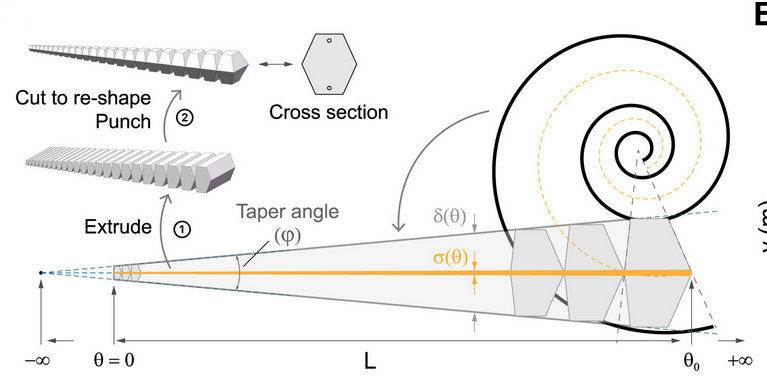
\includegraphics[width=0.7\textwidth]{Figures/draw_solidworks.png}
                \caption{Construction du doigt en "dépliant" la spirale logarthimique \cite{wang_spirobs_2025}}
                \label{fig:draw_solidworks}
            \end{figure}

        Pour dessiner le doigt sur SolidWorks, nous prenons exemple sur la figure \ref{fig:draw_solidworks}. Nous optons néanmoins pour un bossage extrudé à la place de la révolution. Il est désormais question de traduire le formalisme mathématique de la spirale logarthmique en côte des différentes rainures qui composent le doigt (voir figure \ref{fig:draw_solidworks}).
        
        Pour lier la forme en spirale logarithmique du robot aux dimensions (hauteur et longueur) de chaque rainure, nous utilisons le formalisme de la figure \ref{fig:draw_solidworks}.

        On donne l'angle de conicité :

        \begin{equation}
        \phi = 2\arctan \left(
            \frac{\frac{1}{2}\delta(\theta)}{L(-\infty, \theta)}
            \right) = 2 \arctan\left(\frac{b(e^{2\pi b}-1)}{\sqrt{b^2+1} \left(e^{2\pi b}+1\right)}\right)
        \label{angle_de_conicite}
        \end{equation}

        Avec :

        \begin{itemize}
            \item l'épaisseur du robot à l'angle $\theta$ : $\delta(\theta) = ae^{(b\theta + 2\pi)} - ae^{b\theta}$
            \item la longueur du robot entre $[-\infty,\theta]$ : $L(-\infty, \theta) = \int_{-\infty}^{\theta} \sqrt{r_c^2 + \left(\frac{dr}{d\theta}\right)^2} \, d\theta = \frac{r_c(\theta)}{b}$.
        \end{itemize}

        Le fait que $\phi$ soit indépendant de $\theta$ signifie que la forme est effilée \cite{wang_spirobs_2025}.

        Enfin, le rapport entre les épaisseurs de deux rainures adjacentes \(\beta\) est donnée par :
        \begin{equation}
        \beta = \frac{\delta(\theta + \Delta\theta)}{\delta(\theta)} = e^{b \Delta\theta}
        \end{equation}
        
        Cela signifie que la taille ou la géométrie d’une unité peut être mise à l’échelle (agrandie ou réduite) par un facteur $\beta$ par rapport à l’unité précédente. Ainsi, il suffit de concevoir une seule unité de base, puis de l’ajuster avec $\beta$ pour créer les unités adjacentes.

        \subsubsection{Création d'un matériau TPU}

        \subsubsection{Simulation via \textit{SolidWorks Simulation}}

            On crée une nouvelle étude statique. \texttt{Déplacements imposés} permet de définir les conditions limites (géométrie fixe = encastrement). \textit{Chargements externes} permet d'appliquer des forces. Enfin, il faut créer un maillage puis appuyer sur exécuter.

            Pour lancer plusieurs simulation, on utilise étude de conception. On rajoute une variable qu'on lie à la force et que l'on fait varier entre 1 N et 20 N, avant de créer un nouveau capteur sur le maximum de la contrainte de Von-Mises.
        
    \bibliographystyle{IEEEtran}
    \bibliography{references}

\end{document}